\subsection{Módulo Printer}
	\label{sec:printer}
	
	El módulo Printer (ver Figura \ref{fig:GeneralSystem}) realiza la conversión de cada elemento de un vector de M elementos hexadecimales (\textit{packet}[M], M elementos de 4 bits) en caracteres hexadecimales (1 byte). Cada elemento del vector es analizado en cada ciclo de reloj (clk\_i) y demultiplexado, de manera tal de convertir un elemento por vez, para luego enviar el byte correspondiente al módulo UART para su posterior transmisión al exterior. El diagrama de bloques de la máquina de estados finitos con camino de datos se muestra en la Figura \ref{fig:Printer_module}.
	
	\begin{figure}[H]
		\centering
		\includegraphics[width=1\textwidth]{Figuras/Printer_module.png}
		\centering\caption{FSMD del módulo \textit{Printer}.}
		\label{fig:Printer_module}
	\end{figure}
	
	En cada ciclo de reloj el módulo \textit{Printer} demultiplexa el vector \textit{packet}[M] para obtener un elemento lógico que procesar, según el valor del contador vigente, que se incrementa en cada ciclo, hasta un máximo de M-1. Si el elemento \textit{packet}[i] es un valor hexadecimal, se enviará un byte equivalente en ASCII. Por ejemplo, se enviará un byte equivalente al 'A' ASCII si el elemento \textit{packet}[i] es una 'A' hexadecimal.
	
	Cada dos ciclos de reloj el módulo \textit{Printer} genera un pulso para habilitar el envío del último byte generado. Junto con el caracter se envía la señal \textit{wr\_uart} para indicarle a la UART que ese dato debe ser guardado en la FIFO de salida y la señal \textit{processed} para indicarle al módulo \textit{Detector} que se pueden procesar nuevas tramas. El ciclo de procesamiento de la trama a transmitir se describe el diagrama de estados de la Figura \ref{fig:Printer_FSMD}.
	
	\begin{figure}[H]
		\centering
		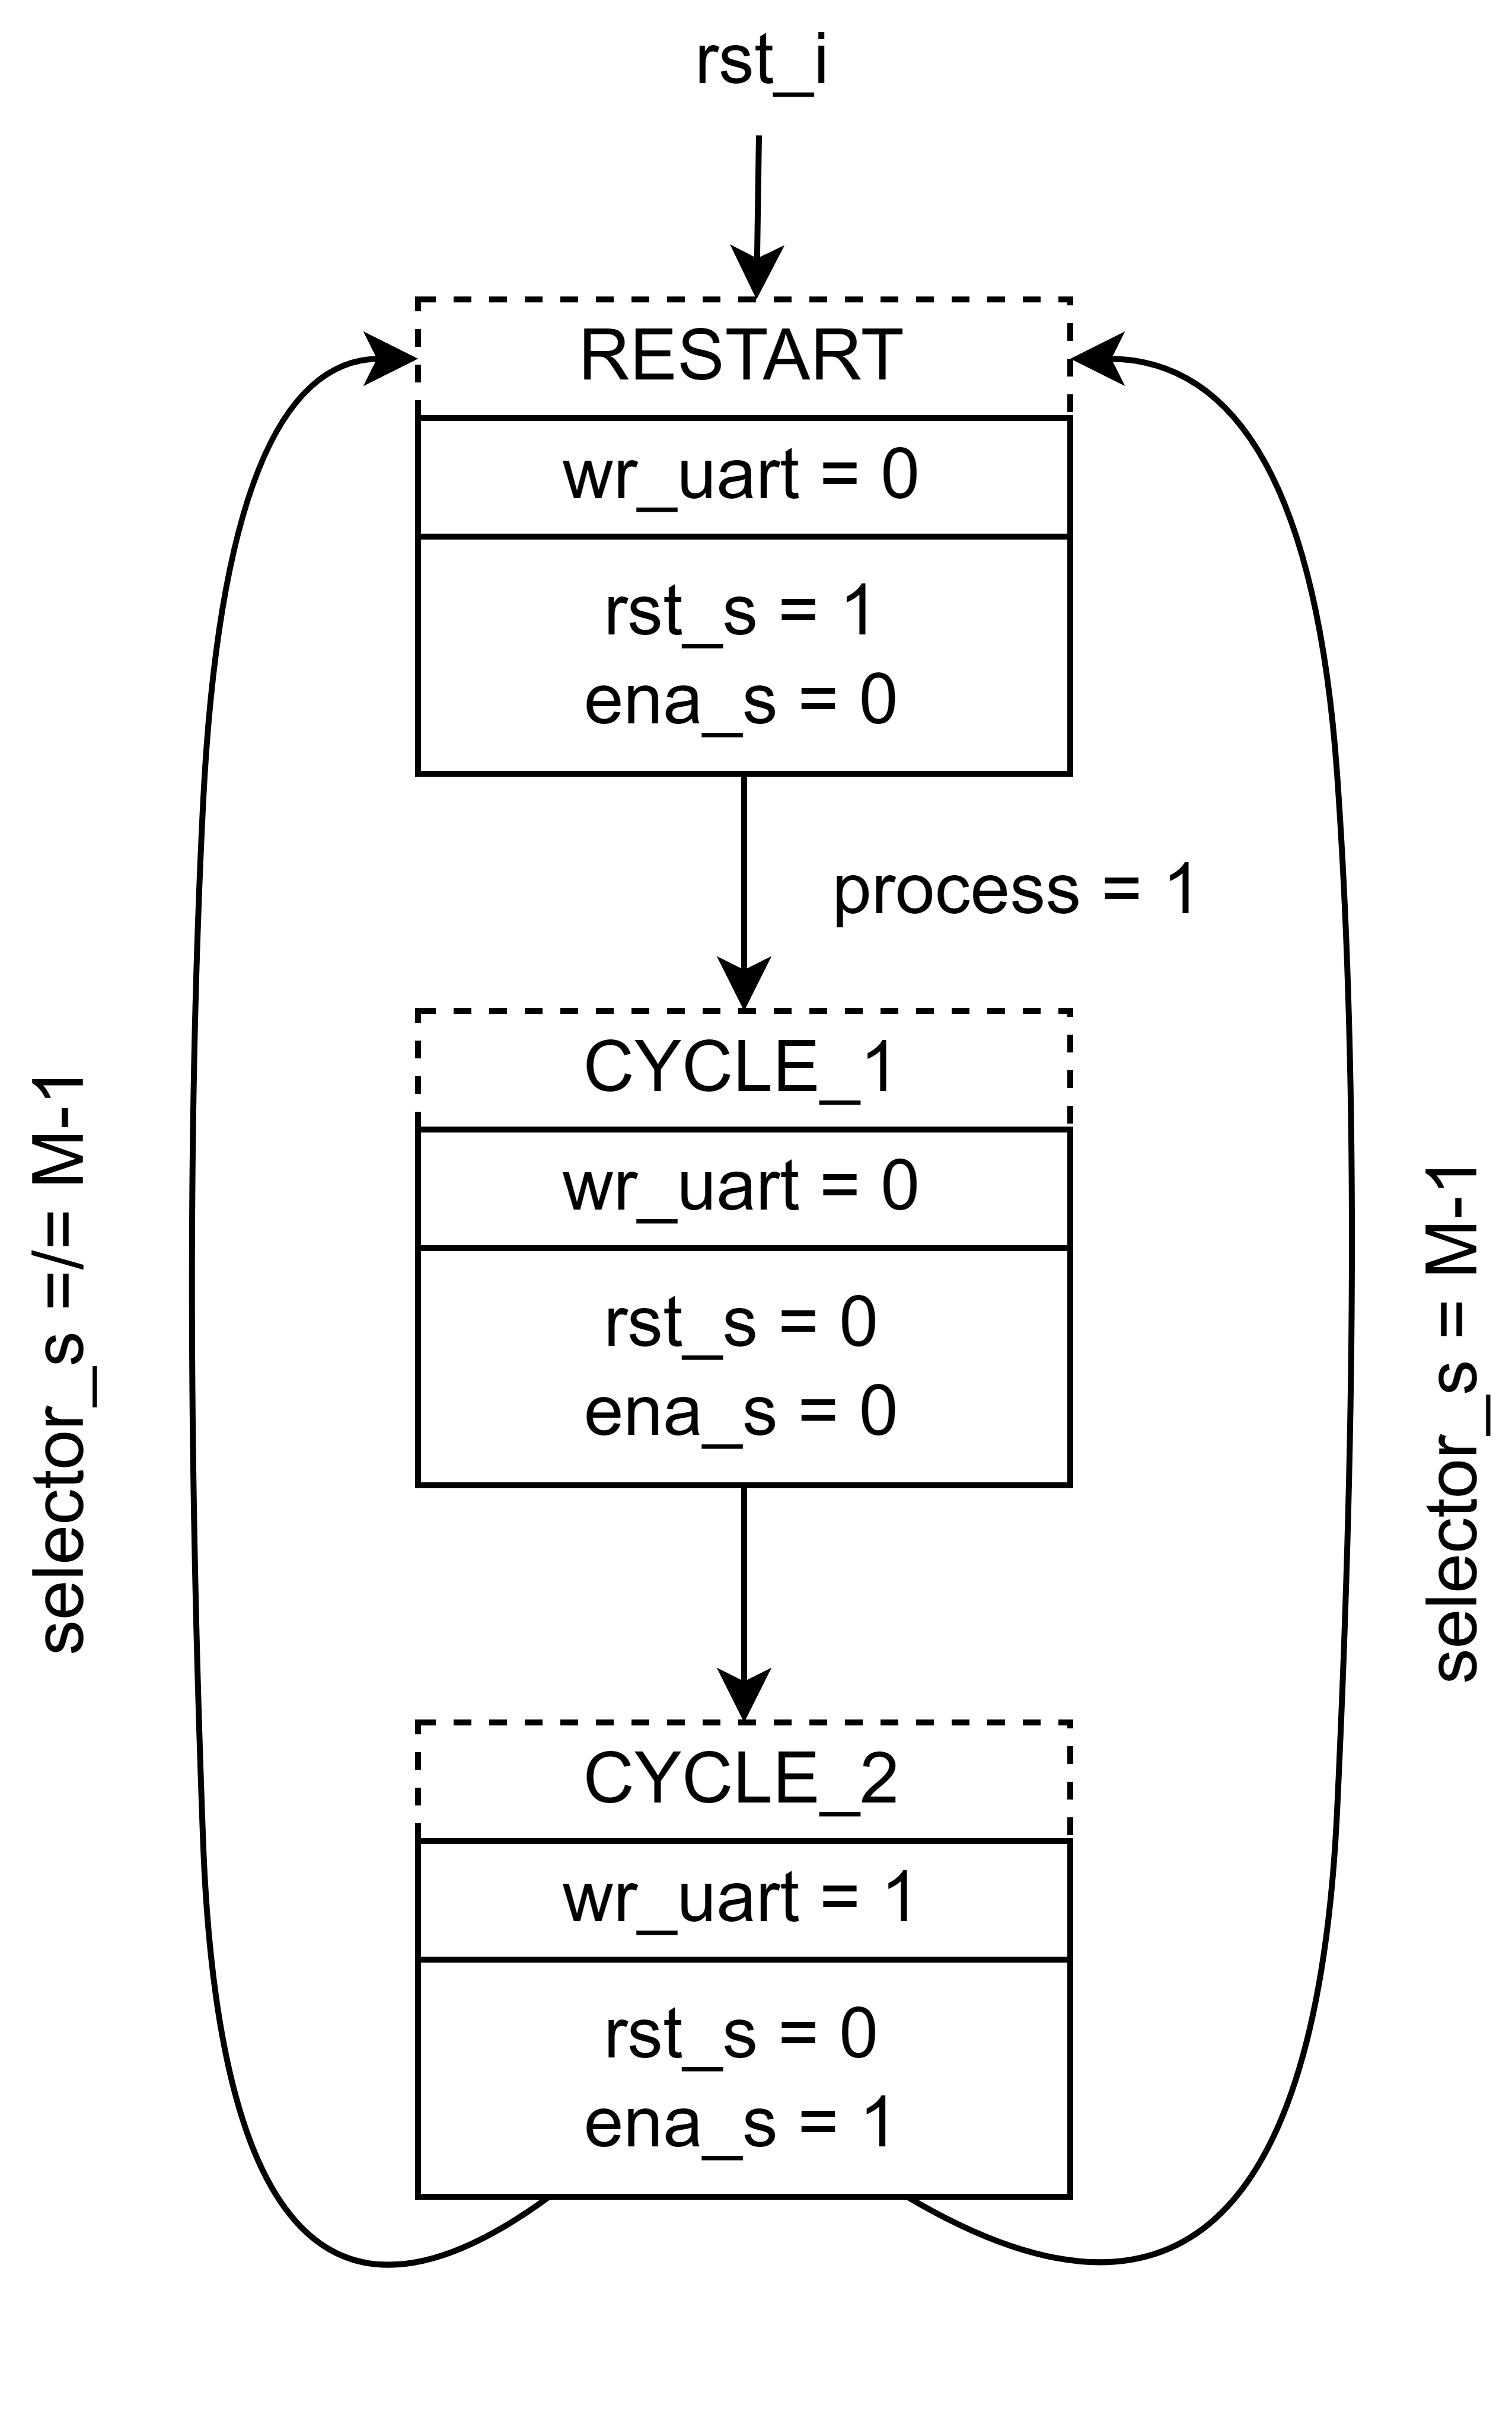
\includegraphics[width=0.8\textwidth]{Figuras/Printer_FSMD.png}
		\centering\caption{Diagrama de estados del módulo \textit{Printer}.}
		\label{fig:Printer_FSMD}
	\end{figure}
	
	El módulo \textit{Printer} inicia por detecto en el estado \textit{restart}, a la espera de recibir la señal \textit{process} del módulo \textit{Encoder}. Se tienen dos estados (\textit{cycle\_1} y \textit{cycle\_2}) para generar el pulso de reloj necesario para mantener sincronizadas las tramas. Cuando el contador haya recorrido los M elementos de \textit{packet}[M], el módulo vuelve al estado \textit{restart}, para esperar una nueva señal \textit{process} para volver a procesar una nueva trama de datos.
	
	Si la trama recibida es incorrecta, o si ya fue impresa, entonces la señal \textit{process} será '0' y el modulo \textit{Printer} dejará de enviar datos a la UART. Si la señal \textit{process} mantiene un estado lógico positivo, el proceso de impresión continuará hasta que la UART indique que no pueda recibir mas datos o que alguna etapa previa informe de algún error en el proceso.